\documentclass[10pt,twocolumn,letterpaper]{article}

% \usepackage[review]{cvpr}      % To produce the REVIEW version
% \usepackage{cvpr}              % To produce the CAMERA-READY version
\usepackage[pagenumbers]{cvpr}   % To force page numbers, e.g. for an arXiv version

\usepackage{CJKutf8}
\usepackage{graphicx}
\usepackage{amsmath}
\usepackage{amssymb}
\usepackage{booktabs}
\usepackage[dvipsnames]{xcolor}
\usepackage[pagebackref,breaklinks,colorlinks]{hyperref}

% Support for easy cross-referencing
\usepackage[capitalize]{cleveref}
\crefname{section}{Sec.}{Secs.}
\Crefname{section}{Section}{Sections}
\Crefname{table}{Table}{Tables}
\crefname{table}{Tab.}{Tabs.}

\usepackage{tikz}
\usetikzlibrary{shapes.geometric, arrows}
\tikzstyle{startstop} = [rectangle, rounded corners, minimum width=3cm, minimum height=1cm,text centered, draw=black, fill=red!30]
\tikzstyle{io} = [trapezium, trapezium left angle=70, trapezium right angle=110, minimum width=3cm, minimum height=1cm, text centered, draw=black, fill=blue!30]
\tikzstyle{process} = [rectangle, minimum width=3cm, minimum height=1cm, text centered, draw=black, fill=orange!30]
\tikzstyle{decision} = [diamond, minimum width=3cm, minimum height=1cm, text centered, draw=black, fill=green!30]
\tikzstyle{arrow} = [thick,->,>=stealth]


%%%%%%%%% PAPER ID
\def\cvprPaperID{Team 23}
\def\confName{CVPR}
\def\confYear{2022}


\begin{document}

%%%%%%%%% TITLE
\title{Abnormal Gait Detection for Medical Application using AI Technology Integrated Wearable Devices}

\author{
    \begin{CJK*}{UTF8}{bkai}
        徐卓朗
    \end{CJK*}
    P76095018\\
    National Cheng Kung University\\
    {\tt\small p76095018@gs.ncku.edu.tw}
    \and
    \begin{CJK*}{UTF8}{bkai}
        胡雋
    \end{CJK*}
    P46104293\\
    National Cheng Kung University\\
    {\tt\small P46104293@gs.ncku.edu.tw}
    \and
    \begin{CJK*}{UTF8}{bkai}
        彭煜博
    \end{CJK*}
    P76111123\\
    National Cheng Kung University\\
    {\tt\small p76111123@gs.ncku.edu.tw}
}
\maketitle

%%%%%%%%% ABSTRACT
\begin{abstract}
\label{sec:abstract}

% \textcolor{blue}{
    Among Parkinson’s disease (PD) motor symptoms, freezing of gait (FOG) may be the most incapacitating. FOG episodes may result in falls and reduce patients’ quality of life. However, Freezing attacks can be mitigated or prevented with external intervention, such as visual or auditory cues activated by FOG prediction and detection systems.
    In this term project, we implement a simple classifier for detecting and predicting FOG episodes in patients. This model is trained using accelerometer data which information should be considered from the previous and current signal windows. We use Long Short-Term Memory (LSTM)~\cite{10.1162/neco.1997.9.8.1735} for our basic structure as deep learning methods are advantageous when dealing with time-series data, such as sensor data.
    This research aimed to determine if LSTM can detect and predict FOG from accelerometer data alone, specifically for use in a real-time wearable system.
% }

\end{abstract}

%%%%%%%%% BODY TEXT
\section{Introduction}
\label{sec:intro}

\begin{figure}[t]
    \centering
    \fbox{
        \rule{0pt}{2in} 
        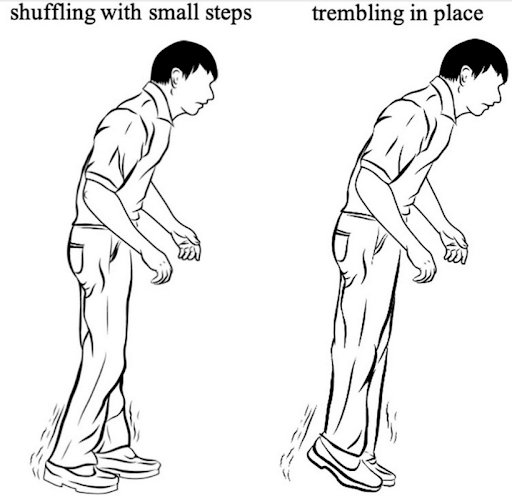
\includegraphics[width=.9\linewidth]{./images/symptoms.png}
    }
    \caption{A schematic diagram of FOG episodes.}
    \label{fig:f1}
\end{figure}

\begin{figure}[t]
    \centering
    \fbox{
        \rule{0pt}{2in} 
        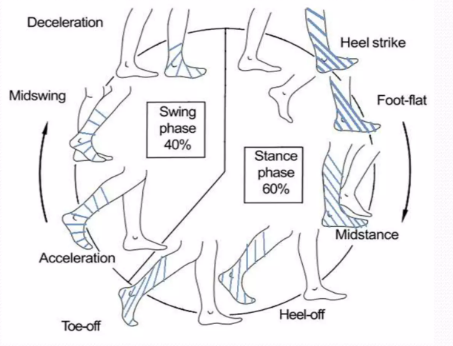
\includegraphics[width=.9\linewidth]{./images/cycle.png}
    }
    \caption{A period of human's GC.}
    \label{fig:f2}
\end{figure}

Parkinson’s disease causes uncontrollable movements which are due to brain disorders. With the progression of this disease, patients can suffer from difficulty walking and talking, and mental and behavioral changes. The most common motor symptoms of Parkinson’s disease are tremor, rigidity, bradykinesia, and postural instability. Among these motor symptoms, freezing of gait (FOG) may be the most incapacitating. FOG episodes may result in falls and reduce patients’ quality of life. However, Freezing attacks can be mitigated or prevented with external intervention, such as visual or auditory cues activated by FOG prediction and detection systems~\cite{10.1016/j.jneurol.2019.01.003}.

Though Parkinson’s disease is the most common among elder people, there are no specific tests to diagnose Parkinson’s disease. The diagnosis of Parkinson’s disease is based on the patient’s medical history, physical examination, and laboratory tests. For example, the patient will be asked to walk on a treadmill, and the doctor will observe the patient’s walking. If the patient has a left foot injury, his center of gravity will be concentrated on the right foot, and his stride may be shorter. If a 100-meter runner, his stride will be solid and hefty. Besides, his toes will need to afford the whole body weight. If a person is about to fall, his steps will suddenly appear disordered. If a right-brain stroke patient, his left toe will land first while walking; meanwhile, the center of gravity will bias toward the right side of the body (Figure \ref{fig:f1}). After these simple testing procedures, the doctor can judge the patient's physical state.

To make these trivial observations more accurate, we use a wearable device to collect the patient's walking data. With the thank of previous research, we can use the data to predict the patient's physical state. For example, the data can be used to predict the patient's gait cycle (GC)~\cite{8540355, gcdef2011}. The GC refers to when a person's heel touches the ground until the same heel touches the ground again. The process can divide into three phases, Stance phase, Swing phase, and Double limb support (Figure \ref{fig:f2}). Observing the changes in foot position during the GC can help estimate a person's physical state, predict the dangers encountered, and issue timely help or medical services~\cite{CAMPS2018119}.

It is worth noting that although the above description is desirable, the first problem we will encounter when conducting gait detection research is how to effectively collect pace data and use appropriate algorithms to perform calculations. In addition, it is necessary to define this experimental subject of our works clearly. Therefore, to solve these problems, we have to conduct a systematic analysis, and the next section will introduce how we carried out this project.

%------------------------------------------------------------------------
\begin{figure}[t]
    \centering
    \fbox{
        \rule{0pt}{2in} 
        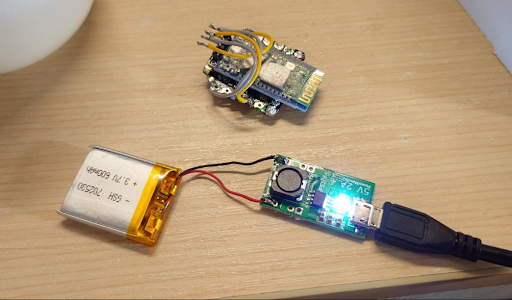
\includegraphics[width=.9\linewidth]{./images/device_apart.png}
    }
    \caption{Materials of the device.}
    \label{fig:f3}
\end{figure}

\begin{figure}[t]
    \centering
        \rule{0pt}{2in}
        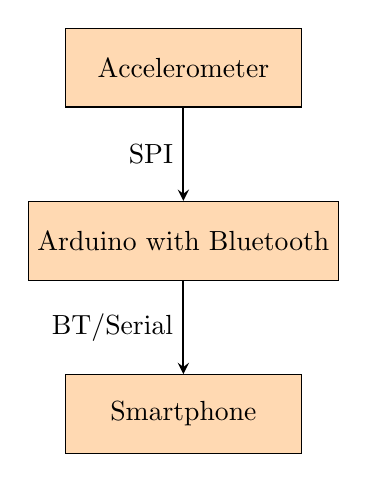
\begin{tikzpicture}[node distance=2cm]
            \node (entity1) [process] {Accelerometer};
            \node (entity2) [process, below of=entity1, yshift=-0.2cm] {Arduino with Bluetooth};
            \node (entity3) [process, below of=entity2, yshift=-0.2cm] {Smartphone};
            \draw [arrow] (entity1) -- node[anchor=east] {SPI} (entity2);
            \draw [arrow] (entity2) -- node[anchor=east] {BT/Serial} (entity3);
        \end{tikzpicture}
    \caption{Data flow of the device operation.}
    \label{fig:f4}
\end{figure}

\section{System framework}
\label{sec:framework}

This project will dedicate in four parts: \textbf{device design}, \textbf{data collection}, \textbf{model training}, and \textbf{validation}. The following sections will introduce the details of each part.

Device design includes the design of the wearable device and the connection to the computation device. The wearable device consists of a microcontroller unit (MCU), an accelerometer, a Bluetooth module, and a battery management system~\cite{pardoel2019wearable} (Figure \ref{fig:f3}). The MCU chip is used to control the accelerometer and Bluetooth module. The accelerometer is used to collect pacing data. The connection between the wearable device and the computation device, for instances, a smartphone, is established by Bluetooth. Our wearable device is designed to be worn on the ankle. The collected data will be sent to the computation device for further processing. The simple design of the device is shown in Figure \ref{fig:f4}.

Data collection operates two collection methods: our designed wearable device and a built-in smartphone application for a few experiments. For example, the sensor can receive acceleration data on three dimensions (x, y, z)-axis from the examinee's foot while he is walking. This collected data is then buffered and sent to our computation devices which will later be processed during data preprocessing. In this project, the examinees will be our team members with intentionally abnormal walking gaits.

Model training is the process of training a model to classify the collected data. We will use the collected data to train a classification network where a classifier can identify which form of data is \textit{Normal} or \textit{Abnormal}.~\cite{s21020614, 8789488}, we will first use a simple LSTM model to classify the data and then use a more complex model to improve the accuracy of the classification.

Validation consists of a patient to see if our model can provide real-time feedback for the patient. For the doctor, we will provide a dashboard to show the patient's current physical state and the predicted physical state. The dashboard will also show the patient's walking data and the predicted walking data. The doctor can use this dashboard to monitor the patient's physical state and predict the patient's physical state.

%-------------------------------------------------------------------------
\begin{figure}[t]
    \centering
    \fbox{
        \rule{0pt}{2in} 
        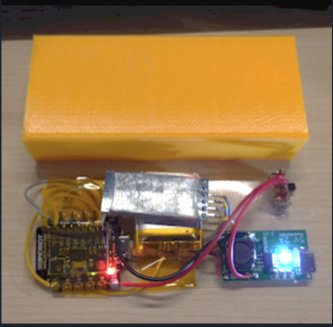
\includegraphics[width=.9\linewidth]{./images/device.png}
    }
    \caption{Our designed accelerometer stick.}
    \label{fig:f5}
\end{figure}

\begin{figure}[t]
    \centering
    \fbox{
        \rule{0pt}{2in} 
        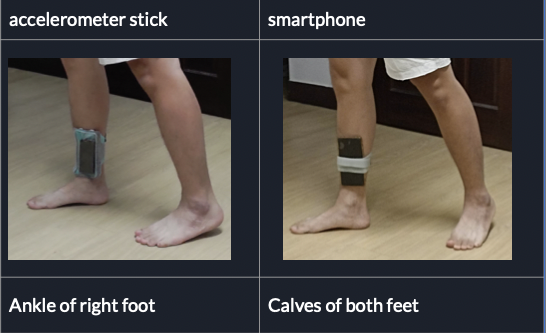
\includegraphics[width=.9\linewidth]{./images/placing.png}
    }
    \caption{The way we adopt in the collection.}
    \label{fig:f6}
\end{figure}

\section{Materials and Methods}
\label{sec:materials}

\subsection{Data Collection}
\label{sec:data_collection}

% \textcolor{blue}{
    Data collection will be done using two methods. One is using the smartphone built in accelerometer and a Arduino powered accelerometer (Figure \ref{fig:f5}) and gyroscope module. We plan that smart phone device will be placed on our calves of both feet and Arduino powered accelerometer be placed on the ankle of right foot simultaneously (Figure \ref{fig:f6}) and then both hardwares will send the collected data to the computer for further processing.
    The smartphone built in accelerometer is a MEMS (Micro Electro Mechanical System) accelerometer. It is a sensor that can measure acceleration forces in three dimensions. The Arduino module is a MPU6050 module. It is a 6-axis motion tracking device that combines a 3-axis gyroscope and a 3-axis accelerometer. The Arduino module is powered by a 3.3V voltage regulator. The Arduino module is connected to the smartphone via Bluetooth. The smartphone will send the data to the computer via Bluetooth. 
% }

\begin{figure}[t]
    \centering
    \fbox{
        \rule{0pt}{2in} 
        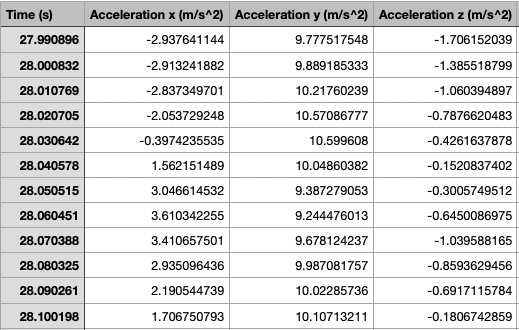
\includegraphics[width=.9\linewidth]{./images/device_data.png}
    }
    \caption{Raw data collected from our designed device.}
    \label{fig:f7}
\end{figure}

\begin{figure}[t]
    \centering
    \fbox{
        \rule{0pt}{2in} 
        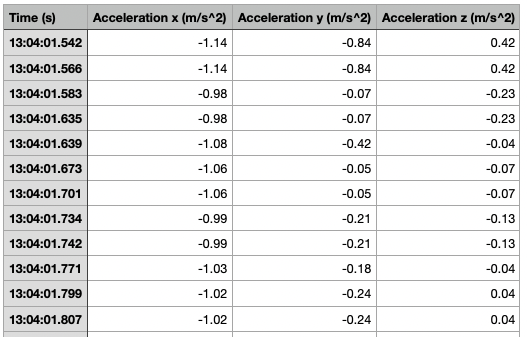
\includegraphics[width=.9\linewidth]{./images/phone_data.png}
    }
    \caption{Raw data collected from smartphone built in accelerometer.}
    \label{fig:f8}
\end{figure}

\subsection{Data structure and preprocessing}
\label{sec:data_structure}

% \textcolor{blue}{
    After collection of the data, we need to preprocess the data. As we have collected data from two different devices, we need to combine these two data sets into one data set. Of course, in order to remove the noise of artifacts, we trimmed the data sets to 10 seconds per data. These data will be stored in a CSV file and we check every data file required with four same columns, \textit{Time}, \textit{Acceleration x}, \textit{Acceleration y}, \textit{Acceleration z}.

    The most complicated part of this procedure is to combine these two data sets. We have collected 10 seconds of data from the Arduino module and 10 seconds of data from the smartphone built in accelerometer. We need to combine these two data sets into one data set. The first problem is that two dataset have different sampling rates, and this caused the problem 2: two data sets have different data points. The Arduino module has 1000 data points. The smartphone built in accelerometer has only 300 data points.

    Finally, we have the data set with 300 data points per data. Each data point will have 4 values. The first value is the time stamp. The second value is the acceleration on the x-axis. The third value is the acceleration on the y-axis. The fourth value is the acceleration on the z-axis (Figure \ref{fig:f7}) (Figure \ref{fig:f8}).
% }

\subsection{Model training}
\label{sec:model_training}

\begin{figure}[t]
    \centering
    \fbox{
        \rule{0pt}{2in} 
        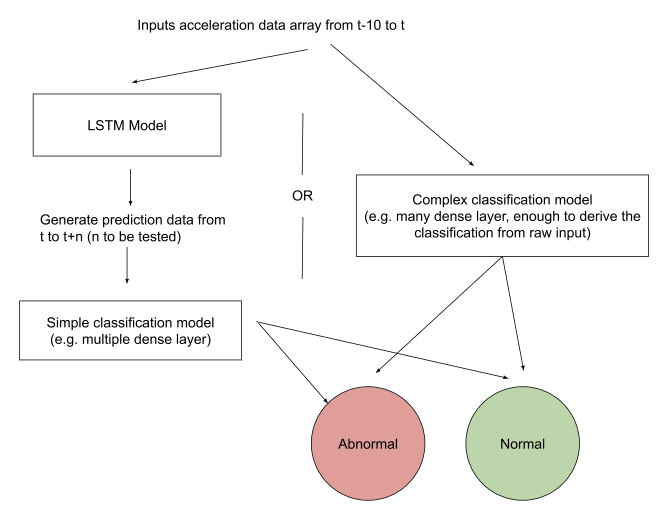
\includegraphics[width=.9\linewidth, height=4.5cm]{./images/model_design.png}
    }
    \caption{Model design for FOG detection.}
    \label{fig:f9}
\end{figure}

\begin{figure}[t]
    \centering
    \fbox{
        \rule{0pt}{2in} 
        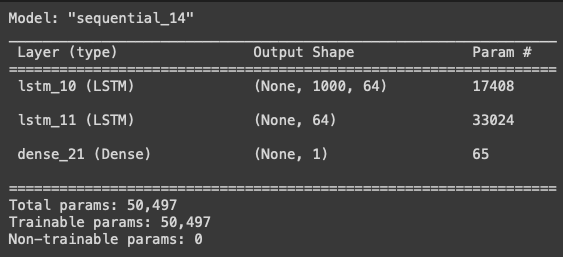
\includegraphics[width=.9\linewidth]{./images/model.png}
    }
    \caption{Pure two layer LSTM model.}
    \label{fig:f10}
\end{figure}

\begin{figure}[t]
    \centering
    \fbox{
        \rule{0pt}{2in} 
        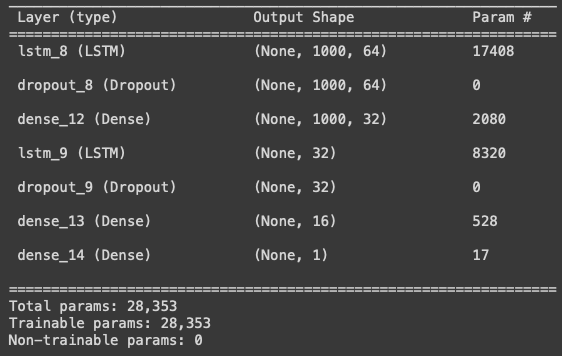
\includegraphics[width=.9\linewidth]{./images/model2.png}
    }
    \caption{Add dropout and dense layer into the model.}
    \label{fig:f11}
\end{figure}

\subsubsection{Long Short-Term Memory (LSTM)}
\label{sec:lstm}

% \textcolor{blue}{
    For FOG detection, LSTM networks were setup using a multiple-input (multiple datapoint) multiple-output (multiple datapoint) architecture in which all datapoints were used as model inputs and each datapoint in the test instances was classified by the model~\cite{Shalin2021}. Each LSTM layer returned the full sequence to the model’s next layer. This allowed the model to classify each timestamp as belonging to the FOG or Non-FOG class. LSTM layers used a hyperbolic tangent (tanh) activation function, followed by a time-distributed fully connected layer (i.e., output at each time step passes through the fully connected layer) with 2 units and Softmax activation. Models were trained with the Adam optimizer, using 0.9 decay rate for the first and 0.999 decay rate for the second moment estimates, and a cross entropy loss function.
% }

\subsubsection{Our model}
\label{sec:our_model}

% \textcolor{blue}{
    Before we start training, we search for some proposed papers, try to find some basic model for FOG detection. Consider with our data structure, we simply designed two way to train the model. The first way is LSTM model. The second way is CNN model (Figure \ref{fig:f9}). Apparaently, the LSTM model is more suitable for our data structure.

    We proposed two basic model for FOG detection. First model is shown in Figure \ref{fig:f10}. The model is a pure two layer LSTM model. The first layer has 128 units and the second layer has 64 units. Second model is shown in Figure \ref{fig:f11}. The model is a two layer LSTM model with dropout and dense layer.~\cite{10.1162/neco.1997.9.8.1735} The first layer has 64 units and the second layer has 32. The dropout rate is 0.2 and the dense layer has 2 units with Relu activation. Both models are trained with 20 epochs and the batch size is 32. The model is trained with the Adam optimizer, using 0.9 decay rate for the first and 0.999 decay rate for the second moment estimates, and a cross entropy loss function.
% }

\section{Results and Discussion}
\label{sec:result}

\begin{figure}[t]
    \centering
    \fbox{
        \rule{0pt}{2in} 
        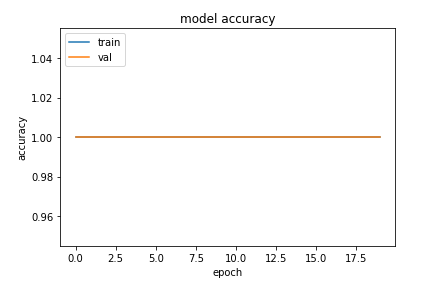
\includegraphics[width=.9\linewidth, height=4.5cm]{./images/model_acc.png}
    }
    \caption{Model 1 accuracy.}
    \label{fig:f12}
\end{figure}

\begin{figure}[t]
    \centering
    \fbox{
        \rule{0pt}{2in} 
        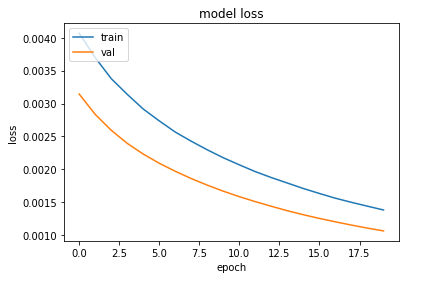
\includegraphics[width=.9\linewidth, height=4.5cm]{./images/model_loss.png}
    }
    \caption{Model 1 loss.}
    \label{fig:f13}
\end{figure}

\begin{figure}[t]
    \centering
    \fbox{
        \rule{0pt}{2in} 
        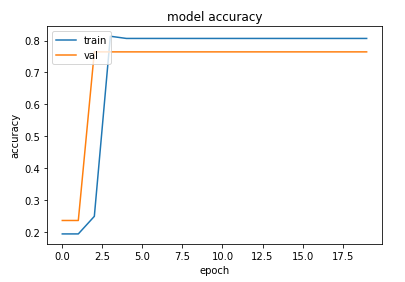
\includegraphics[width=.9\linewidth, height=4.5cm]{./images/model2_acc.png}
    }
    \caption{Model 2 accuracy.}
    \label{fig:f14}
\end{figure}

\begin{figure}[t]
    \centering
    \fbox{
        \rule{0pt}{2in} 
        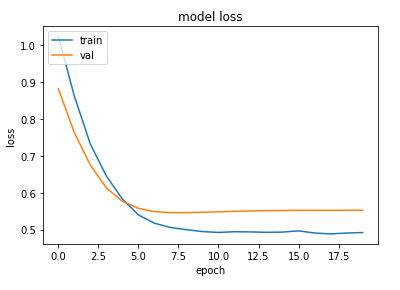
\includegraphics[width=.9\linewidth, height=4.5cm]{./images/model2_loss.png}
    }
    \caption{Model 2 loss.}
    \label{fig:f15}
\end{figure}

% \textcolor{blue}{
    In our first proposed model 1, we can see that the accuracy is almost 1.0 and the loss can be reduced to 0.001 or lower, which means the model is trained well. For a deeper analysis, because of not enough training data and data imbalancing, the model easily goes overfitting on specific data distributed.

    In our second proposed model 2, we modify the model by adding dropout and dense layer. We simplify the model proposed by Hochreiter \etal~\cite{10.1162/neco.1997.9.8.1735}, so it is more lightweight and easier to train. We can see that the accuracy is almost goes well after the third epoch and the loss reduced to 0.4, the result seems more reasonable.

    In view of the above results, we further did some data augmentation to improve the model performance. We collect more abnormal data. Now, we increase the epoch to 100. The result is shown in Figure \ref{fig:f16}. The result is better than the previous one. First, the accuracy has drastically oscillation before epoch 40. After epoch 40, the accuracy becomes stable. Second, the loss is also stable after epoch 40. The result shows that the model is trained well and the data augmentation is effective.
% }

\begin{figure}[t]
    \centering
    \fbox{
        \rule{0pt}{2in} 
        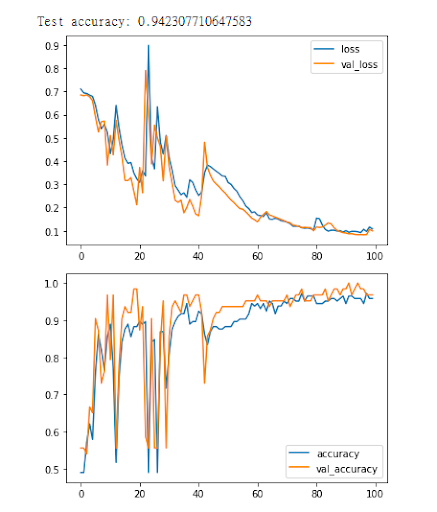
\includegraphics[width=.9\linewidth, height=9cm]{./images/revised.png}
    }
    \caption{Data augmentation result.}
    \label{fig:f16}
\end{figure}

%-------------------------------------------------------------------------
\section{Proposed Design}
\label{sec:design}

% \textcolor{blue}{
    The device will be mounted on the ankle section of the patient and the test subjects. Acceleration data (together with other sensor data) will be collected and compared by the AI model~\cite{10.1007/978-3-319-59147-6_30}. Fully Connected Network (FCN) and LSTM will be used to evaluate which can better generate data from least data point and perform classification of whether the test subject has certain kinds of diseases that might cause walking gait issues. For example, there are results showing that FOG can be detected by just observing the walking gait of the test subject using a foot pressure sensor or accelerometer.
% }

%-------------------------------------------------------------------------
\section{Future Work}
\label{sec:future_work}

% change above to: paragraph of text
% \textcolor{blue}{
    Our work had achieved the goal of detecting FOG by using the accelerometer data. However, there are still some limitations that need to be solved. First, the data segmentation is not automatic: currently, We manually segment the data. Second, the data pre-process is not done: we didn't use peak detection algorithm for preprocessing. Third, the accuracy is not high enough: a more complex model structure design may help. Finally, we need to add a post processing algorithm to filter out noise.
    
    The last but not least, if we want to use this device in the real world, we need to enable realtime classification and realtime warnings. The device should be able to detect whether the test subject has FOG or not. If the test subject has FOG, the device should be able to give a warning to the test subject.

% \begin{itemize}
    % \item \textcolor{blue}{Use InvenSense GY-521 MPU-6050 6DOF to generate Arduino powered Accelerometer.}
    % \item \textcolor{blue}{Collect more patient-specific walking behaviors and use these data to train and test the model.}
    % \item \textcolor{blue}{Calculate the accuracy and the loss function of the model.}
    % \item \textcolor{blue}{Distinguish whether the test subjects have walking gait issues or not.}
    % \item \textcolor{blue}{If it is difficult to classify whether the test subjects are abnormal or not, try to collect other information to improve the recognition.}
    % Automatic Walking / Non-walking data segmentation
    % Data pre-process with peak detection algorithm 
    % Enable realtime classification and realtime warnings
    % Increase accuracy
    % With more complex model structure design and collected data
    % Add a post processing algorithm to filter out noise
% \end{itemize}

%-------------------------------------------------------------------------
\section{Expected results}
\label{sec:results}

A classification network that allows anyone to check their walking gait and provide feedback if an abnormality is detected. The network will be able to detect FOG and other walking gait issues.

%%%%%%%%% REFERENCES
{\small
\bibliographystyle{ieee_fullname}
\bibliography{egbib}
}

\end{document}
